\documentclass[11pt]{standalone}
\usepackage[T1]{fontenc}
\usepackage{pgfplots}
\usepackage{xcolor, colortbl}


\definecolor{sfugrey}{RGB}{253, 252, 247}
\definecolor{sfublack}{RGB}{4, 89, 163}
\definecolor{sfured}{RGB}{251, 180, 98}


\begin{document}
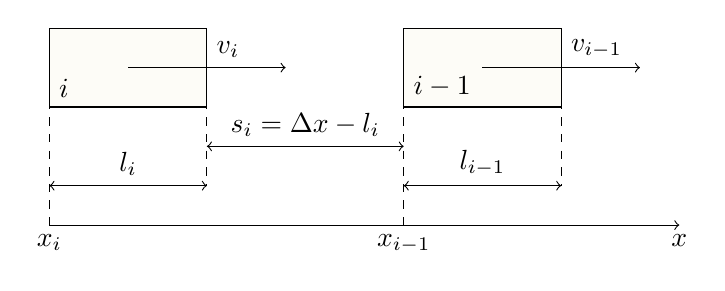
\begin{tikzpicture}
\def\rectanglepath{-- ++(2cm,0cm) -- ++(0cm,1cm) -- ++(-2cm,0cm) -- cycle}
\draw[fill=sfugrey] (0,0) \rectanglepath node[above right, black]{$i$};
\draw[->] (1.0cm,0.5cm) --node[above right]{$v_i$} (3.0cm,0.5cm);
\draw[fill=sfugrey] (4.5,0) \rectanglepath node[above right, black]{$i-1$};
\draw[->] (5.5cm,0.5cm) --node[above right]{$v_{i-1}$} (7.5cm,0.5cm);

\draw[->] (0cm,-1.5cm) -- (8cm,-1.5cm)node[below]{$x$};

\draw[dashed](0.0cm,.5cm) -- (0.0cm,-1.5cm) node[below]{$x_i$};
\draw[dashed](2.0cm,.5cm) -- (2.0cm,-1.0cm);
\draw[<->] (0.0cm,-1.0cm) --node[above]{$l_i$} (2.0cm,-1.0cm);

\draw[dashed](4.5cm,.5cm) -- (4.5cm,-1.5cm) node[below]{$x_{i-1}$};
\draw[dashed](6.5cm,.5cm) -- (6.5cm,-1.0cm);
\draw[<->](4.5cm,-1.0cm) --node[above]{$l_{i-1}$} (6.5cm,-1.0cm);

\draw[<->] (2.0cm,-0.5cm)--node[above]{$s_i = \Delta x - l_i$} (4.5cm,-0.5cm);

\end{tikzpicture}

\end{document}
